\subsection{ORB-SLAM3}

ORB-SLAM3 is a KV-SLAM implementation which is popular in research contexts due to its performance, open source codebase, and usage of methods and techniques that are well-documented and widely understood. Figure \ref{fig:orb-slam3} shows a simplified diagram of the internal processes of ORB-SLAM3, which is a good starting point for understanding the system.

\begin{figure}[!ht]
    \centering
    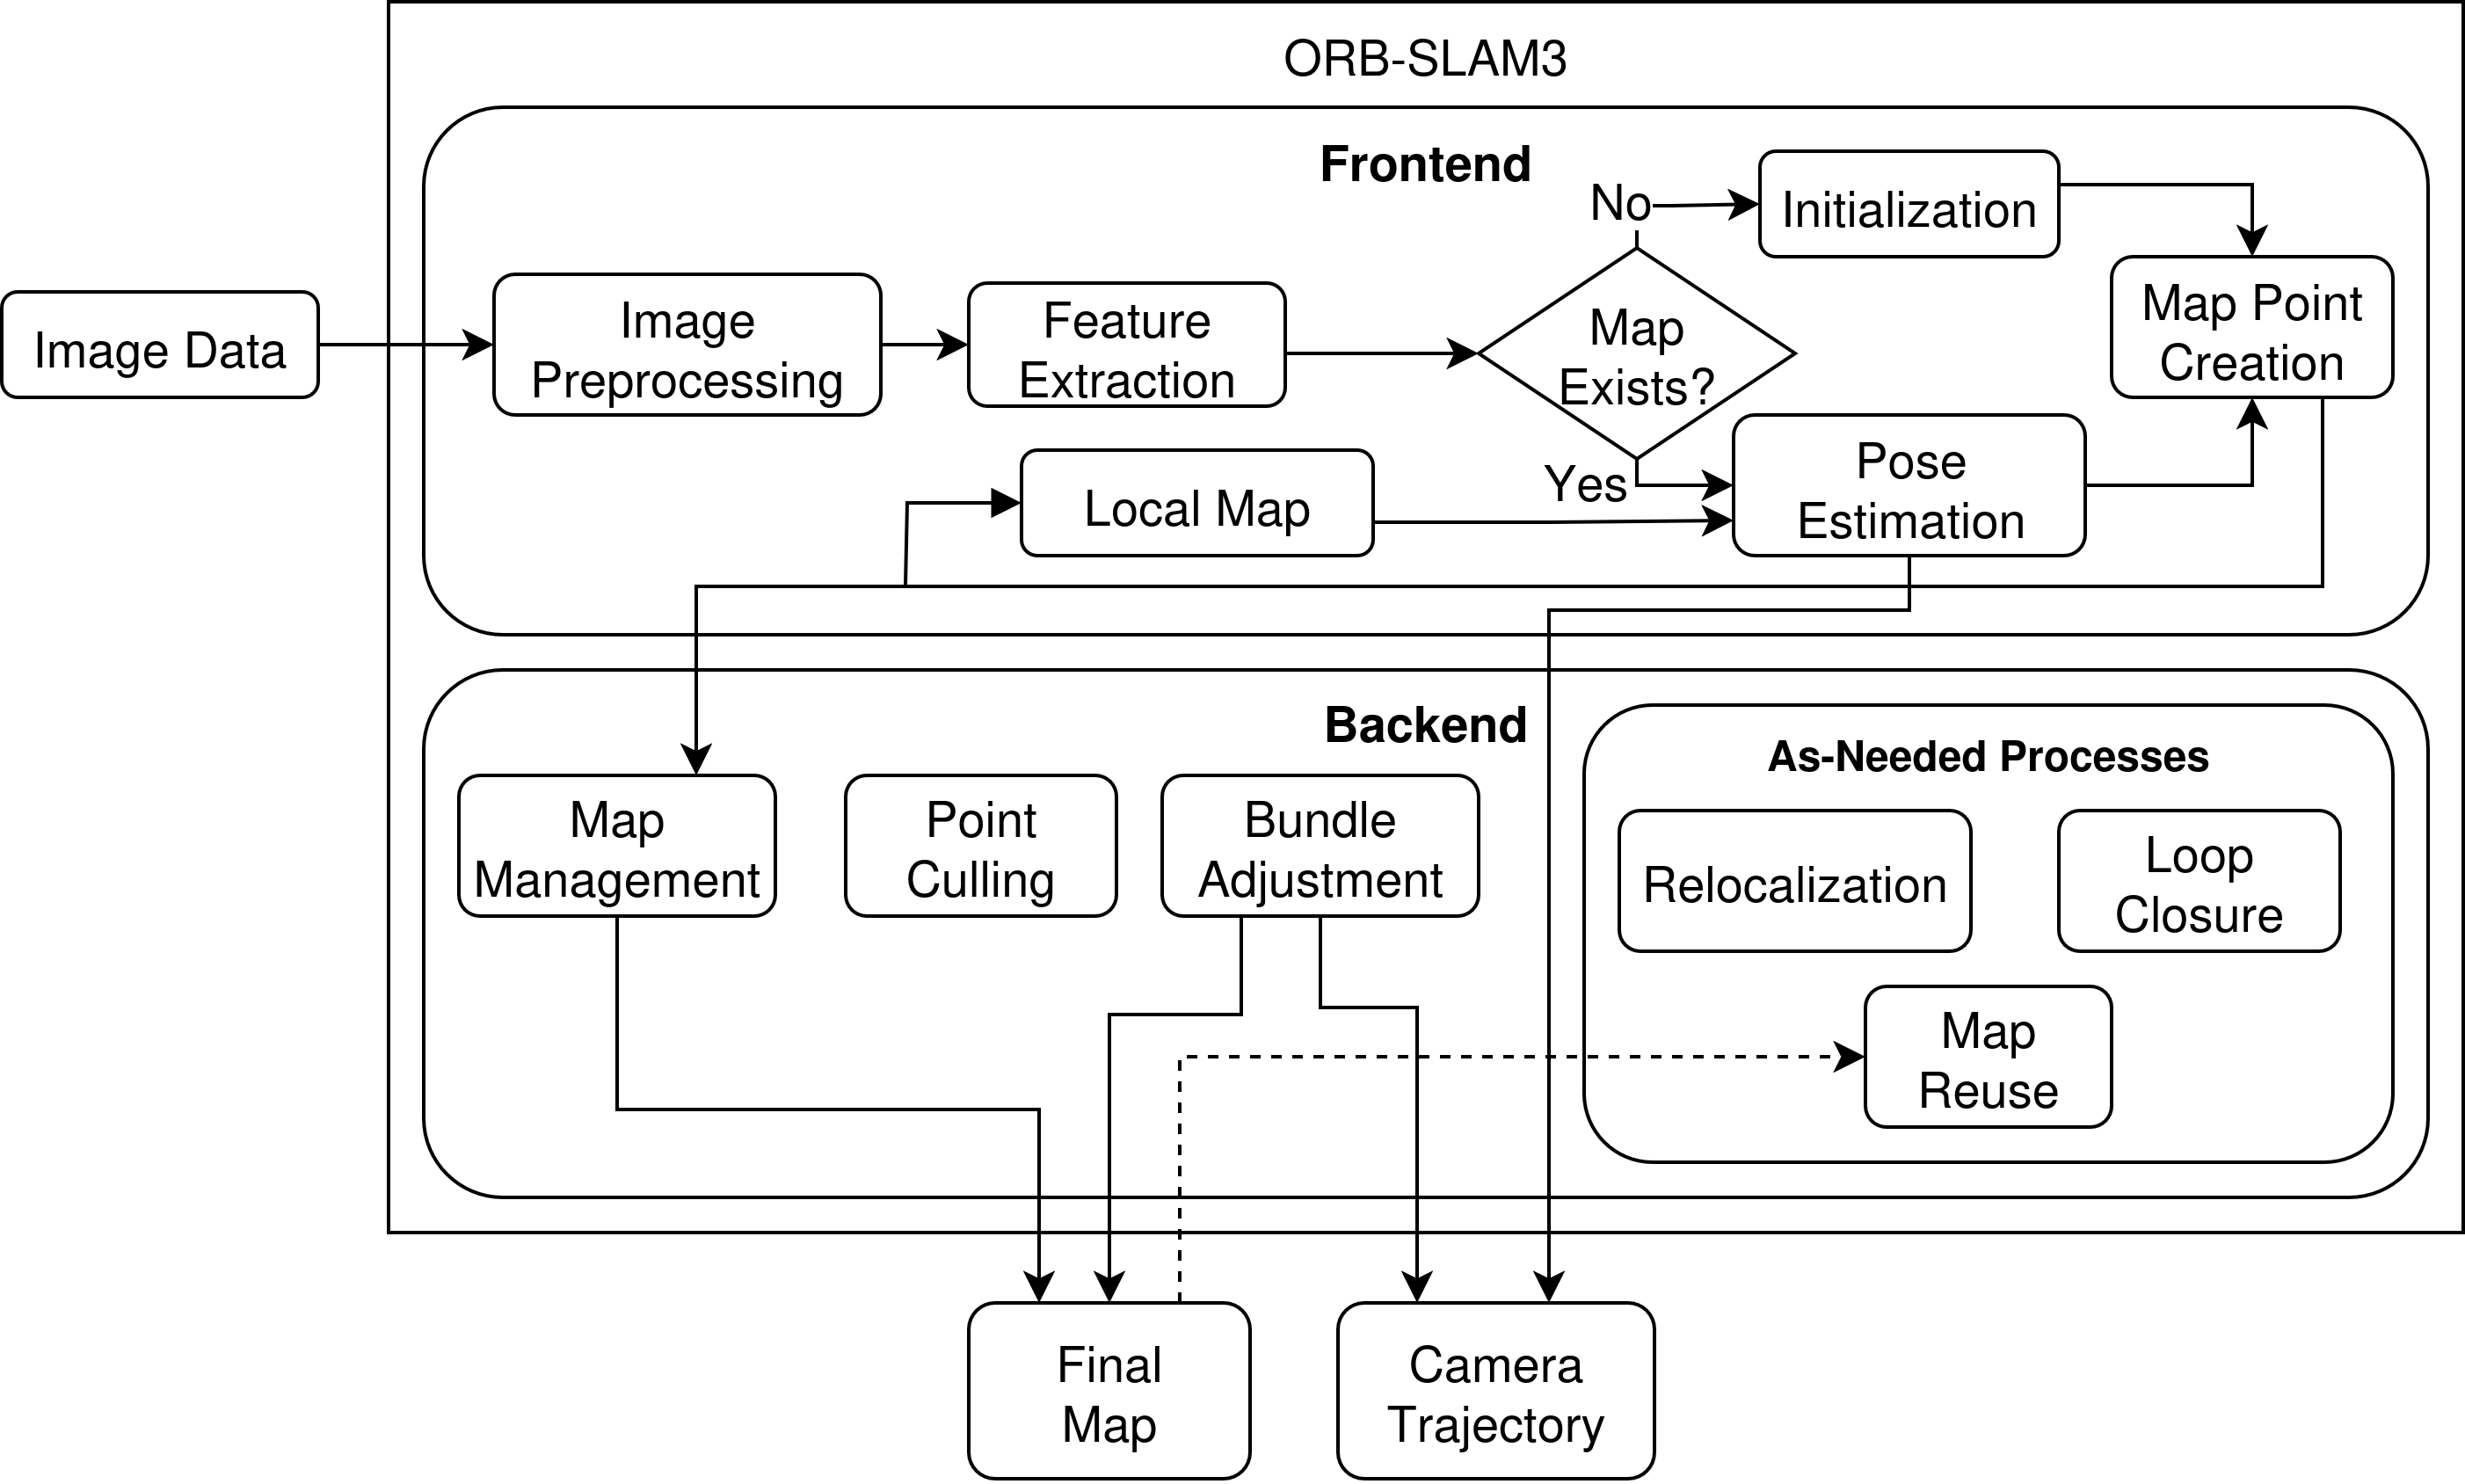
\includegraphics[width=0.9\textwidth]{resources/orb-slam3.png}
    \caption[Simplified ORB-SLAM3 Operational Diagram]{A simplified diagram of the inputs, outputs, and subprocesses of ORB-SLAM3.}
    \label{fig:orb-slam3}
\end{figure}

ORB-SLAM3 splits its operations across multiple threads, allowing it to process images, track map points, and optimize the map concurrently. The system uses popular 